\documentclass[11pt]{beamer} 
\usetheme{PaloAlto}
\usepackage[utf8]{inputenc} 
\usepackage{xeCJK, fontspec, xunicode, xltxtra} 
\usepackage{amsmath} 
\usepackage{amsfonts} 
\usepackage{amssymb} 
\usepackage{graphicx} 
\usefonttheme{serif} 
\setCJKmainfont[BoldFont=STHeiti]{STKaiti} 
\setmonofont{Courier New}
\usecolortheme{crane} 
%\setmainfont{Times}
\usepackage{listings}
\usepackage{xcolor}
\usepackage{hyperref}

\author[赵玉炜]{{\fontspec{Times New Roman}{NJUPT.SAST.ACM组}}\quad 赵玉炜} 
\title{哈希思想} 

%\setbeamercovered{transparent} 
%\setbeamertemplate{navigation symbols}{} 
\logo{
\includegraphics[scale=0.08]{NJUPT-logo.png}} 

%\institute{} 
\date{2018年7月} 
%\subject{} 

\definecolor{Green}{RGB}{60,179,113}
\definecolor{Orange}{RGB}{255,165,0}
\definecolor{Moccasin}{RGB}{255,228,181}
\lstset{
	alsoletter={/},
	basicstyle=\ttfamily,
	breaklines=true,
	keywordstyle={\bfseries\color{Green}},
	frame=shadowbox,
	frameround=tftt,
	rulecolor={\color{Orange}},
	rulesepcolor={\color{Orange}},
	backgroundcolor={\color{Moccasin}},
	emph={bits/stdc++,cout,endl,namespace},
	emphstyle={\bfseries\color{red!80!black}},
	tabsize=4,
	numbers=right,
	numberstyle={\bfseries\tiny\ttfamily},
	numbersep=-0.6em,
	commentstyle={\itshape\color{blue}}
}



\begin{document}

\defverbatim[colored]\cirDemo{
\begin{lstlisting}[language=c++]
#include <bits/stdc++.h>
using namespace std;
int main() {
	/*定义变量s和n并做必要的初始化*/
	int s = 0, n;
	cin >> n; /*输入n*/
	for (int i = 1; i <= n; ++i) {
		s += i;
	} /*对1-n循环累加*/
	cout << s << endl; /*输出s*/
	return 0;
}
\end{lstlisting}
}


\begin{frame}
\titlepage
\end{frame}

%\begin{frame}
%\tableofcontents
%\end{frame}

\section{预备知识}
\begin{frame}[c]
\frametitle{预备知识}
\begin{enumerate}
	\item 循环
	\item 数组
\end{enumerate}
\end{frame}







\section{问题引入}
\subsection{问题1.1}
\begin{frame}[c]\frametitle{问题引入}
\only<1> {
	\begin{block}{{\textbf{问题1.1}\quad 数字查询}}
	输入一个序列$A: a_1, a_2, a_3\ldots a_n$,包含$n$个数字。下面进行$m$次查询,每次查询需要确定一个数字$b_i$在不在序列$A$中。数据范围$1 \leq n,m,a_i,b_i\leq 100$。

	(\textbf{时间限制:} 1000MS,\textbf{空间限制:} 64MB)
	\end{block}

	\begin{block}{\textbf{格式}}
	{\textbf{输入}}-输入共四行,第一行一个数$n$,第二行$n$个数表示序列$A$,第三行一个数$m$,第四行$m$个数给出$m$次询问。

	{\textbf{输出}}-输出$m$行,表示$m$次询问的结果,如果$b_{i}\in A$输出``Yes'',否则输出``No''。
	\end{block}
}
%--------------------------------------
\only<2> {
	\begin{block}{{\textbf{问题1.1}\quad 数字查询}}
	输入一个序列$A: a_1, a_2, a_3\ldots a_n$,包含$n$个数字。下面进行$m$次查询,每次查询需要确定一个数字$b_i$在不在序列$A$中。数据范围$1 \leq n,m,a_i,b_i\leq 100$。

	(\textbf{时间限制:} 1000MS,\textbf{空间限制:} 64MB)
	\end{block}

	\textbf{暴力求解法} \quad 把$n$个数保存在数组$A$中,然后对于$m$次询问的每一个数,都用遍历$A$数组的方法检验这个数是否在$A$中。渐进时间复杂度$O(mn^2)$。

}
\end{frame}
\subsection{问题1.2}
\begin{frame}[c]\frametitle{问题引入}
\onslide<1-> 
	\begin{block}{{\textbf{问题1.2}\quad 数字查询}}
	输入一个序列$A: a_1, a_2, a_3\ldots a_n$,包含$n$个数字。下面进行$m$次查询,每次查询需要确定一个数字$b_i$在不在序列$A$中。数据范围$1 \leq n,m,a_i,b_i\leq 10^6$。

	(\textbf{时间限制:} 1000MS,\textbf{空间限制:} 64MB)
	\end{block}
	相较上一个问题,数据范围发生了改变。
\onslide<2->

	\textbf{考虑1}\quad 数据范围$10^6$如果使用$O(mn^2)$的算法会超时。

\onslide<3->

	\textbf{考虑2}\quad $10^6$个int类型的数据所占空间大小约为3.8MB。

\onslide<4->

	\textbf{考虑3}\quad 是否可以开一个$10^6+1$长度的int数组,如果$i\in A$,那么下标为$i$的元素设为1,反之设为0?
\onslide<5->{\color{red!80!black}(渐进时间复杂度$O(\max\{n,m\})$,正解)。}
\end{frame}

\section{哈希思想}
\begin{frame}
\frametitle{哈希表与哈希思想}
\onslide<1->
\quad 刚刚我们使用的数组叫做\textbf{哈希表}。

\onslide<2->
\begin{center}
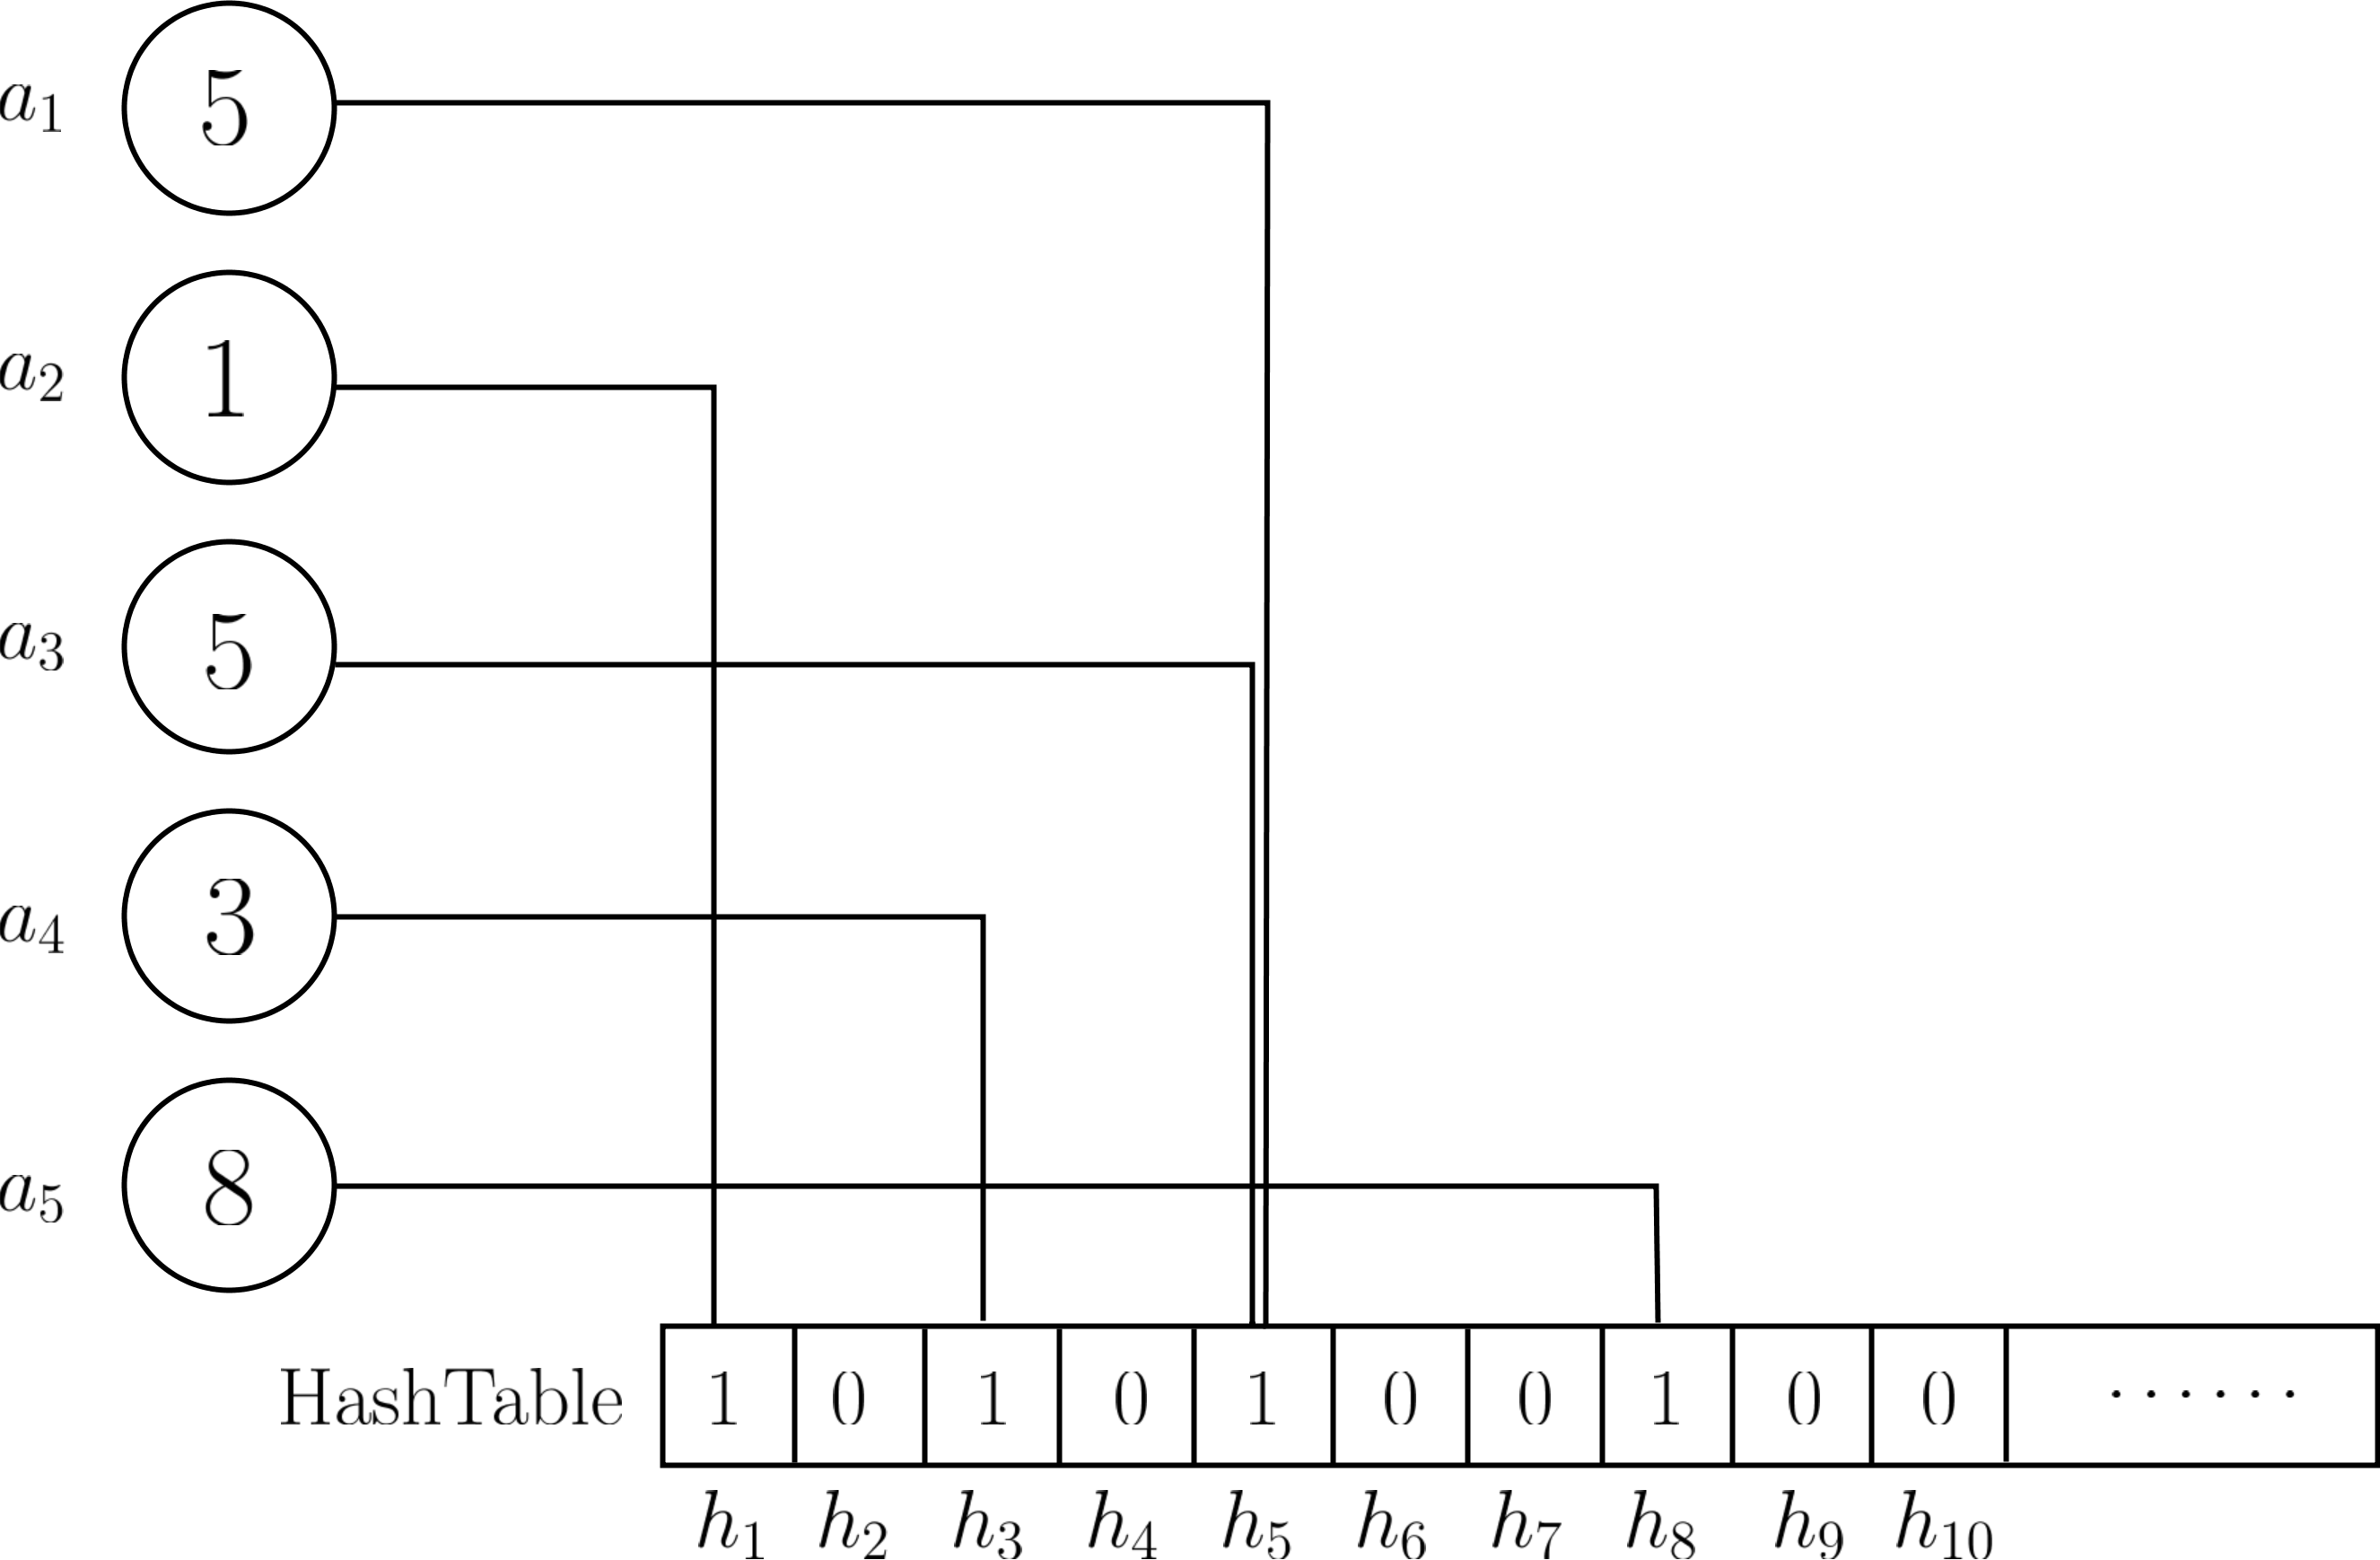
\includegraphics[scale=0.1]{HashTable.png}
\end{center}


\end{frame}



\end{document}